\chapter{Figures}


\begin{figure}[H]
  \centering
  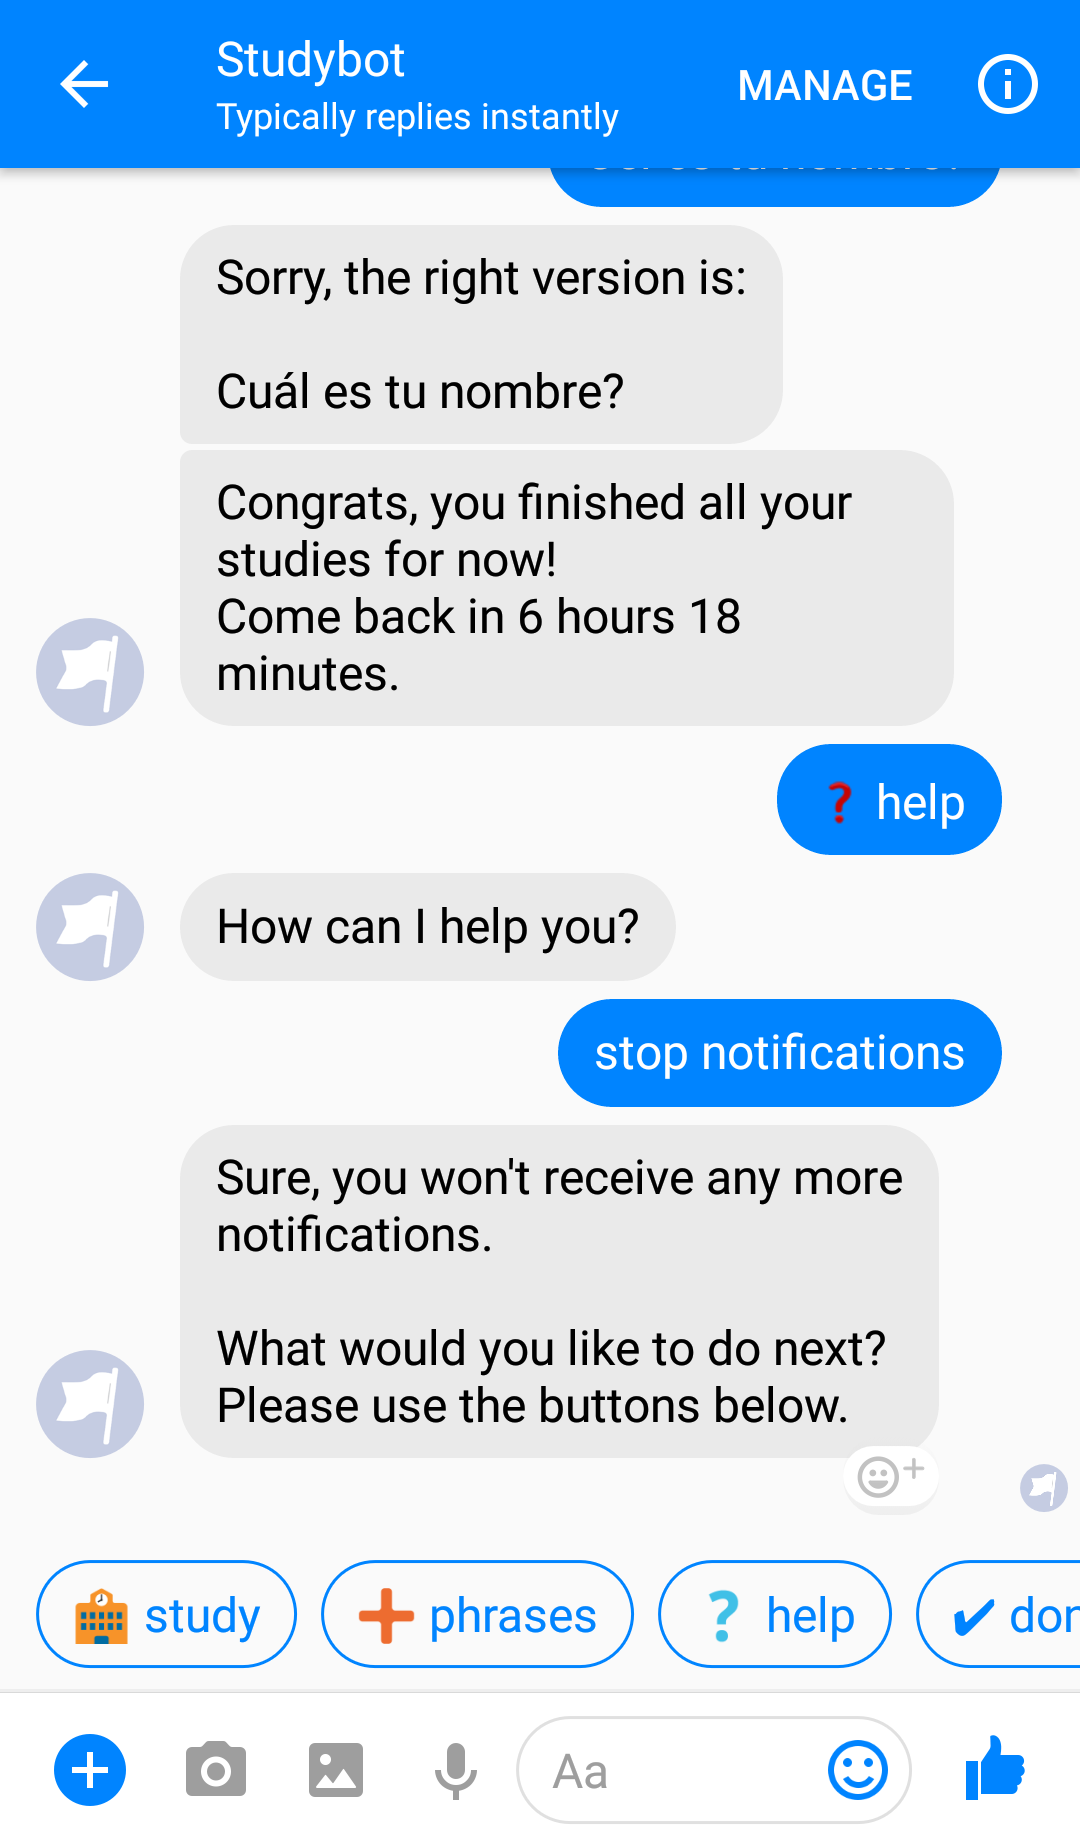
\includegraphics[width=0.3\textwidth]{images/interface/10-disable-notify.png}
	\caption{Disable notifications}
	\label{fig:10-disable-notify}
\end{figure}


\chapter{Call Graphs}

\begin{figure}[H]
  \centering
  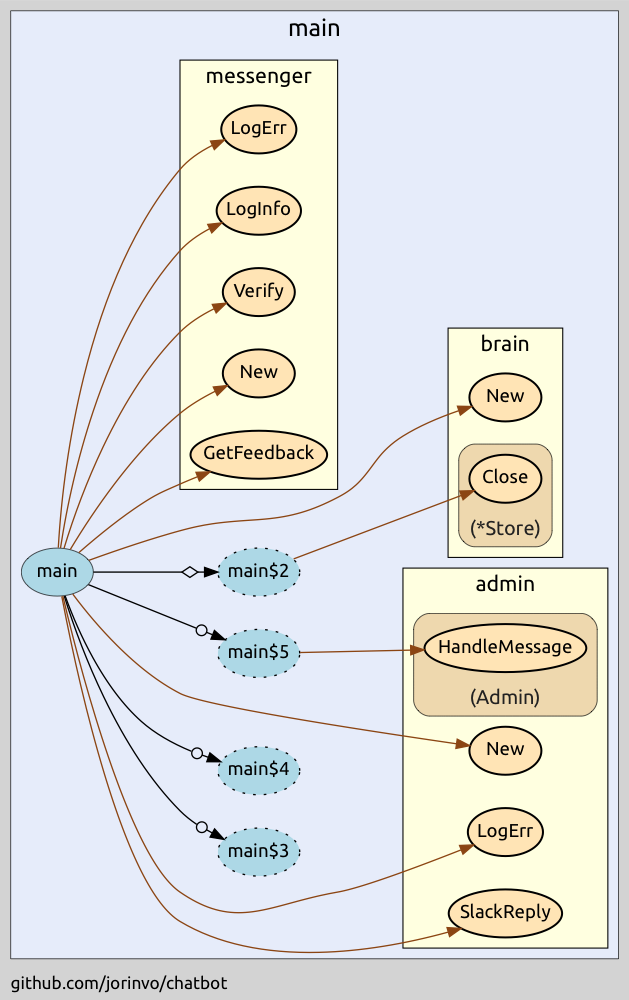
\includegraphics[height=14cm]{images/call-graph-main.png}
	\caption{Call Graph of package main}
  \label{a:call-graph}
\end{figure}

\begin{figure}[H]
  \centering
  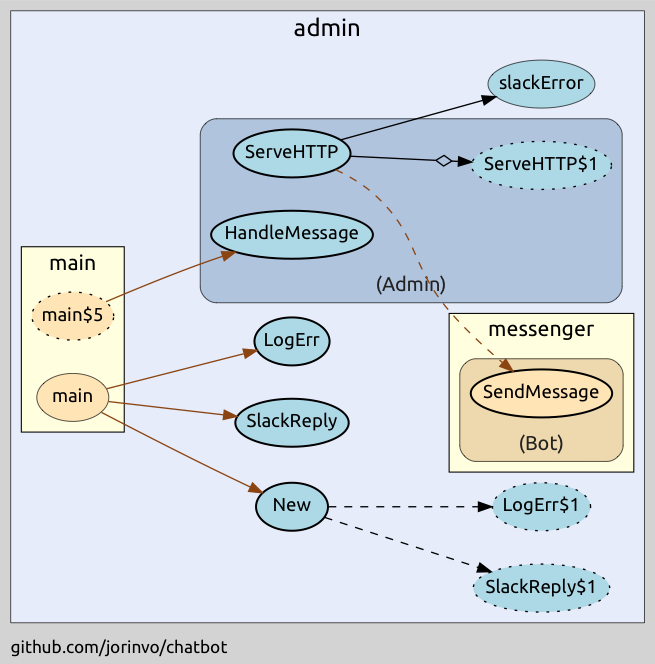
\includegraphics[height=8cm]{images/call-graph-admin.png}
	\caption{Call Graph of package admin}
\end{figure}

\begin{figure}[H]
  \centering
  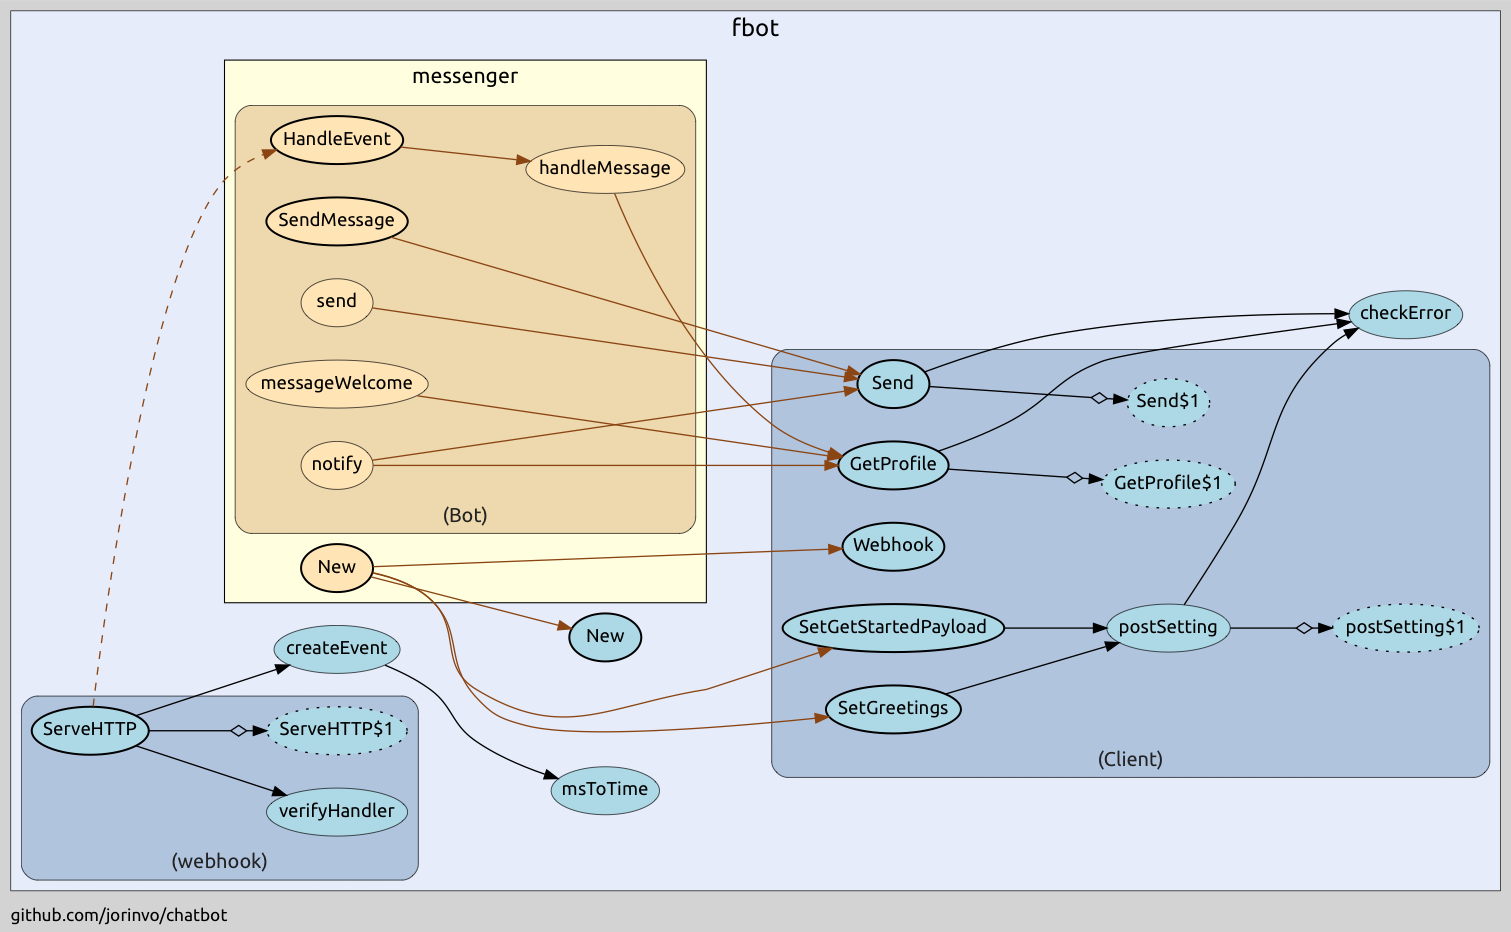
\includegraphics[width=\textwidth]{images/call-graph-fbot.png}
	\caption{Call Graph of package fbot}
\end{figure}

\chapter{Documentation}
\label{a:docs}

\lstset{
	extendedchars=true,
	numbers=left,
	numberstyle=\tiny,
	breakautoindent  = true,
	breakindent      = 2em,
	breaklines       = true,
}

\begin{lstlisting}[
  caption={Command line interface usage information},
  basicstyle=\scriptsize\ttfamily
]
Studybot

Usage: chatbot [flags]

Studybot uses BoltDB as a database.
Data is stored in a single file. No external system is needed.
However, only one application can access the database at a time.

Studybot starts a server to serve a webhook handler that can be registered as a Messenger bot.
The server is HTTP only and a proxy server should be used to make the bot available on
a public domain, preferably HTTPS only.

An admin server runs on a separate port.
It should be proxied and secured via HTTPS + basic auth.
The admin server provides an endpoint to fetch backups of the database.
Further, it provides an endpoint that can be registered as Slack Outgoing Webhook.

When users send feedback to the bot, the messages are forwarded to Slack
and admin replies in Slack are send back to the users.


Flags:
  -admin int
    	Port admin interface listens on. (default 8081)
  -db string
    	Required. Path to BoltDB file. Will be created if non-existent.
  -port int
    	Port Facebook webhook listens on. (default 8080)
  -slackhook string
    	Required. URL of Slack Incoming Webhook. Used to send user messages to admin.
  -slacktoken string
    	Token for Slack Outgoing Webhook. Used to send admin answers to user messages.
  -token string
    	Required. Messenger bot token.
  -verify string
    	Required. Messenger bot verify token.
\end{lstlisting}


\pagebreak
\begin{lstlisting}[
  caption={Go documentation for package messenger},
  basicstyle=\scriptsize\ttfamily
]
package messenger
    import "github.com/jorinvo/chatbot/messenger"

    Package messenger implements the Messenger bot and handles all the user
    interaction.

FUNCTIONS

func GetFeedback(f chan<- Feedback) func(*Bot)
    GetFeedback sets up user feedback to be sent to the given channel.

func LogErr(l *log.Logger) func(*Bot)
    LogErr is an option to set the error logger of the bot.

func LogInfo(l *log.Logger) func(*Bot)
    LogInfo is an option to set the info logger of the bot.

func Notify(b *Bot)
    Notify enables sending notifications when studies are ready.

func Setup(b *Bot)
    Setup sends greetings and the getting started message to Facebook.

func Verify(token string) func(*Bot)
    Verify is an option to enable verification of the webhook.

TYPES

type Bot struct {
    http.Handler
    // contains filtered or unexported fields
}
    Bot is a messenger bot handling webhook events and notifications. Use
    New to setup and use register Bot as a http.Handler.

func New(store brain.Store, token string, options ...func(*Bot)) (Bot, error)
    New creates a Bot. It can be used as a HTTP handler for the webhook. The
    options Setup, LogInfo, LogErr, Notify, Verify, GetFeedback can be used.

func (b Bot) HandleEvent(e fbot.Event)
    HandleEvent handles a Messenger event.

func (b Bot) SendMessage(id int64, msg string) error
    SendMessage sends a message to a specific user.

type Feedback struct {
    ChatID   int64
    Username string
    Message  string
}
    Feedback describes a message from a user a human has to react to
\end{lstlisting}


\pagebreak
\begin{lstlisting}[
  caption={Go documentation for package admin},
  basicstyle=\footnotesize\ttfamily
]
package admin
    import "github.com/jorinvo/chatbot/admin"

    Package admin provides an admin server that can be used to make backups
    and to communicate with users via Slack.

FUNCTIONS

func LogErr(l *log.Logger) func(*Admin)
    LogErr is an option to set the error logger.

func SlackReply(token string, fn func(int64, string) error) func(*Admin)
    SlackReply isa n option to enable /slack to receive replies from Slack.
    token is used to validate posts to the webhook. fn is called with a
    chatID and a message.

TYPES

type Admin struct {
    // contains filtered or unexported fields
}
    Admin is a HTTP handler that can be used for backups and to communicate
    with users via Slack.

func New(store brain.Store, slackHook string, options ...func(*Admin)) Admin
    New returns a new Admin which can be used as an http.Handler.

func (a Admin) HandleMessage(id int64, name, msg string)
    HandleMessage can be called to send a user message to Slack.

func (a Admin) ServeHTTP(w http.ResponseWriter, r *http.Request)
    ServeHTTP serves the different endpoints the admin server provides.
\end{lstlisting}


\pagebreak
\begin{lstlisting}[
  caption={Go documentation for package fbot},
  basicstyle=\scriptsize\ttfamily
]
package fbot
    import "github.com/jorinvo/chatbot/fbot"

    Package fbot can be used to communicate with a Facebook Messenger bot.
    The supported API is limited to only the required use cases and the data
    format is abstracted accordingly.

FUNCTIONS

func API(url string) func(*Client)
    API can be passed to New for sending requests to a different URL. Must
    not contain trailing slash.

TYPES

type Button struct {
    // Text is the text on the button visible to the user
    Text string
    // Payload is a string to identify the quick reply event internally in your application.
    Payload string
}
    Button describes a text quick reply.

type Client struct {
    // contains filtered or unexported fields
}
    Client can be used to communicate with a Messenger bot.

func New(token string, options ...func(*Client)) Client
    New rerturns a new client with credentials set up.

func (c Client) GetProfile(id int64) (Profile, error)
    GetProfile fetches a user profile for an ID.

func (c Client) Send(id int64, message string, buttons []Button) error
    Send a text message with a set of quick reply buttons to a user.

func (c Client) SetGetStartedPayload(p string) error
    SetGetStartedPayload displays a "Get Started" button for new users. When
    a users pushes the button, a postback with the given payload is
    triggered.

func (c Client) SetGreetings(greetings map[string]string) error
    SetGreetings sets the text displayed in the bot description. Pass a map
    of locale to greeting text. Include "default" locale as fallback for
    missing locales.

func (c Client) Webhook(handler func(Event), verifyToken string) http.Handler
    Webhook returns a handler for HTTP requests that can be registered with
    Facebook. The passed event handler will be called with all received
    events.

type Event struct {
    // Type helps to decide how to react to an event.
    Type EventType
    // ChatID identifies the user. It's a Facebook user ID.
    ChatID int64
    // Time describes when the event occured.
    Time time.Time
    // Text is a message a user send for EventMessage and and error description for EventError.
    Text string
    // Payload is a predefined payload for a quick reply or postback sent with EventPayload.
    Payload string
}
    Event contains information about a user action.

type EventType int
    EventType helps to distinguish the different type of events.

const (
    // EventUnknown is the default and will be used if none of the other types match.
    EventUnknown EventType = iota
    // EventMessage is triggered when a user sends Text, stickers or other content.
    // Only text is available at the moment.
    EventMessage
    // EventPayload is triggered when a quickReply or postback Payload is sent.
    EventPayload
    // EventRead is triggered when a user read a message.
    EventRead
    // EventError is triggered when the webhook is called with invalid JSON content.
    EventError
)

type Profile struct {
    Name     string  `json:"first_name"`
    Locale   string  `json:"locale"`
    Timezone float64 `json:"timezone"`
}
    Profile has all public user information we need; needs to be in sync
    with the URL abouve.
\end{lstlisting}


\pagebreak
\begin{lstlisting}[
  caption={Go documentation for package brain},
  basicstyle=\scriptsize\ttfamily
]
package brain
    import "github.com/jorinvo/chatbot/brain"

    Package brain handles all business logic of Slangbrain. It handles data
    storage, retrieving and updating. It's independent from the used bot
    platform and user interaction.

TYPES

type Mode int
    Mode is the state of a chat. We need to keep track of the state each
    chat is in.

const (
    // ModeMenu shows the main menu.
    ModeMenu Mode = iota
    // ModeAdd lets the user add new phrases.
    ModeAdd
    // ModeStudy goes to phrases ready to study.
    ModeStudy
    // ModeGetStarted sends an introduction to the user.
    ModeGetStarted
    // ModeFeedback allows the user to send a message that is ready by a human.
    ModeFeedback
)

type Phrase struct {
    Phrase      string
    Explanation string
    Score       int
}
    Phrase describes a phrase the user saved.

type Store struct {
    // contains filtered or unexported fields
}
    Store provides functions to interact with the underlying database.

func New(dbFile string) (Store, error)
    New returns a new Store with a database already setup.

func (store Store) AddPhrase(chatID int64, phrase, explanation string) error
    AddPhrase stores a new phrase.

func (store Store) BackupTo(w http.ResponseWriter)
    BackupTo streams backup as an HTTP response.

func (store Store) Close() error
    Close the underlying database connection.

func (store Store) DeleteChat(chatID int64) error
    DeleteChat removes all records of a given chat.

func (store Store) DeletePhrases(fn func(int64, Phrase) bool) (int, error)
    DeletePhrases removes all phrases fn matches.

func (store Store) DeleteStudyPhrase(chatID int64) error
    DeleteStudyPhrase deletes the phrase the passed user currently has to
    study.

func (store Store) EachActiveChat(fn func(int64)) error
    EachActiveChat runs a function for each chat where the user has been
    active since the last notification has been sent.

func (store Store) FindPhrase(chatID int64, fn func(Phrase) bool) (Phrase, error)
    FindPhrase returns a phrase belonging to the passed user that matches
    the passed function.

func (store Store) GetChatIDs() ([]int64, error)
    GetChatIDs returns chatIDs of all users.

func (store Store) GetMode(chatID int64) (Mode, error)
    GetMode fetches the mode for a chat.

func (store Store) GetNotifyTime(chatID int64) (time.Duration, int, error)
    GetNotifyTime gets the time until the user should be notified to study.
    Returns the time until the next studies are ready and a count of the
    ready studies. The returned duration is always at least dueMinInactive.
    The count is 0 if the chat has no phrases yet.

func (store Store) GetPhrasesAsJSON(chatID int64) (io.Reader, error)
    GetPhrasesAsJSON ...

func (store Store) GetStudy(chatID int64) (Study, error)
    GetStudy returns the current study the user needs to do.

func (store Store) IsSubscribed(chatID int64) (bool, error)
    IsSubscribed checks if a user has notifications enabled.

func (store Store) ScoreStudy(chatID int64, score int) error
    ScoreStudy sets the score of the current study and moves to the next
    study.

func (store Store) SetActivity(chatID int64, t time.Time) error
    SetActivity sets the last time a message was sent to a user.

func (store Store) SetMode(chatID int64, mode Mode) error
    SetMode updates the mode for a chat.

func (store Store) SetRead(chatID int64, t time.Time) error
    SetRead sets the last time the user read a message.

func (store Store) StudyNow() error
    StudyNow resets all study times of all users to now.

func (store Store) Subscribe(chatID int64) error
    Subscribe enables notifications for a user.

func (store Store) Unsubscribe(chatID int64) error
    Unsubscribe disables notifications for a user.

type Study struct {
    // Phrase is the phrase the user needs to guess.
    Phrase string
    // Explanation is the explanation displayed to the user.
    Explanation string
    // Total is the total number of studies ready, including the current one.
    Total int
    // Next contains the time until the next study is available;
    // it's only set if Total is 0.
    Next time.Duration
}
    Study is a study the current study the user needs to answer.
\end{lstlisting}
